\newpage
\begin{center}
	\textbf{\large 1. ОСНОВНЫЕ ПОНЯТИЯ}
\end{center}

\refstepcounter{chapter}
\addcontentsline{toc}{chapter}{1. ОСНОВНЫЕ ПОНЯТИЯ}



\section{Взаимодействие темной материи с веществом}
Для нахождения сечений взаимодействия темной материи с веществом обычно используются эффективные лагранжианы \cite{Fitzpatrick_2013}, соответствующие векторному или скалярному переносчику взаимодействия. В нерелятивистком пределе матричный элемент рассеяния соответствует квантовомеханическому потенциалу взаимодействия. В релятивисткой нормировке для двух частиц массами $m_1,m_2$ он равен 
\begin{equation}
	\label{eq:mat_element}
	\mathcal{M} = 4m_1 m_2 V(\vec{q})
\end{equation}
где $V(\vec{q})$ --- фурье образ от нерелятивисткого потенциала. 

Наиболее простые члены взаимодействия  скалярного ($g\overline{\chi}\chi\overline{\psi}\psi$) или векторного типа ($g\overline{\chi}\gamma^{\mu}\chi\overline{\psi}\gamma_{\mu}\psi$) дают спин-независимый потенциал вида
\begin{eqnarray}
	V(\vec{q}) = g \rightarrow	V(\vec{r}_1,\vec{r}_2) = \cfrac{g}{4\pi}
	\delta^3(\vec{r}_1-\vec{r}_2)
\end{eqnarray}
где $\vec{q}$ --- переданный импульс. Приведем простейшие лагранжианы и потенциалы взаимодействия с нуклоном (обозначим спины нуклона и темной материи как $\vec{S}_{i}$ и  $\vec{S}_{\chi}$)

\begin{table}[ht]
	\begin{center}
		\begin{tabular}{|c|c|c|}
			\hline && \\[-1em] 
			 & $\mathcal{L}_{int}$ & $\hat{V}(\vec{q})$ \\
			\hline && \\[-1em] 
			1 & $g\overline{\chi}\chi\overline{\psi}\psi$ и 	
			$g\overline{\chi}\gamma^{\mu}\chi\overline{\psi}\gamma_{\mu}\psi$ & g \\
			\hline && \\[-1em] 
			2 & $g \overline{\chi}\gamma^5\chi\overline{\psi}\psi$ & $2ig \vec{S}_{\chi}\vec{q}$\\
			\hline && \\[-1em]
			3 & $g \overline{\chi}\chi\overline{\psi}\gamma^5\psi$ & $2ig \vec{S}_{i}\vec{q}$\\
			\hline && \\[-1em]
			4 & $g \overline{\chi}\gamma^5\chi\overline{\psi}\gamma^5\psi$ & $-4g \vec{S}_{i}\vec{q}\vec{S}_{\chi}\vec{q}$\\
			\hline
		\end{tabular}
		\caption{Примеры простейших потенциалов}
	\end{center}		
	\label{tb:potentials}
\end{table}

Выбрав потенциал взаимодействия с протоном/нейтроном, можно найти эффективный потенциал взаимодействия с ядром $\hat{V}_{N}(q)$. Волновые функции ядра и частицы темной материи равны
\begin{equation}
	\begin{cases}
		\ket{\Psi_N} = e^{-i\vec{r}_N \vec{p}} \ket{\psi_N} \\
		\ket{\chi} = e^{-i\vec{r}_{\chi} \vec{k}} \ket{\chi} \\
	\end{cases}
\end{equation}
где $\vec{r}_N$ --- центр масс ядра, $\ket{\psi_N}$ --- волновая функция нуклонов в ядре, $\ket{\chi}$ --- спиновая волновая фунция частицы $\vec{p}$ --- импульс ядра, $\vec{k}$ --- импульс частицы  темной материи. Оператор взаимодействия с нуклоном имеет тензорную структуру вида $\hat{V}_{i}(\vec{q}) = V(\vec{q})^{ab} \hat{F}^{\chi}_a(\vec{S}_{\chi})\hat{F}^{i}_b(\vec{S}_{i})$, гда $a$ и $b$ пробегают либо нулевой индекс, либо векторный индекс. Потенциал взаимодействия с ядром равен сумме потенциалов взаимодействия с нуклонами $\hat{V}_{N} = \sum_i{\hat{V}_{i}(\vec{r}_i + \vec{r}_N - \vec{r}_{\chi})}$, где $\vec{r}_i$ --- положение нуклона относительно центра масс, причем 
\begin{equation}
	\hat{V}_{i}(\vec{r}_i + \vec{r}_N - \vec{r}_{\chi}) = 
	\int{d^3\vec{q}\,' V(\vec{q}\,')^{ab} \hat{F}^{\chi}_a(\vec{S}_{\chi})\hat{F}^{i}_b(\vec{S}_{i})} e^{i\vec{q}(\vec{r}_i + \vec{r}_N - \vec{r}_{\chi})}
\end{equation}
Тогда матричный элемент (или эффективный потенциал) равен 
\begin{equation}
\begin{split}
	\bra{out}\hat{V}_{N}\ket{in} = V(\vec{q})^{ab} \bra{\chi'}\hat{F}^{\chi}_a\ket{\chi} 
	\bra{\psi_N'} \sum_i{e^{i\vec{r}_i\vec{q}}} \hat{F}^{i}_b(\vec{S}_{i})\ket{\psi_N}
\end{split}
\end{equation}

Полный квадрат матричного элемента из \ref{eq:mat_element} получается при усреднении по спинам и равен
\begin{equation}
	|\mathcal{M}|^2 = 16 m_N^2 m_{\chi}^2 V(\vec{q})^{ab} V^*(\vec{q})^{cd} W^{\chi}_{ac} W^{N}_{bd}
\end{equation}
где
\begin{equation}
	W_{ab} = \cfrac{1}{N_i}\sum_{i,f}{\bra{f}F_a\ket{i}\bra{i}F^+_b\ket{f}} 
\end{equation}
В случае спин независимого (SI) или спин зависимого (SD) потенциала получается соответственно
\begin{equation}
	\begin{split}
		W^{\chi SI}_{00} = 1 \\ 
		W^{\chi SD}_{ij} = \frac{S_{\chi}(S_{\chi}+1)}{3} \delta_{ij} \\
	\end{split}
\end{equation}

Для ядра такие факторы усложняются суммой осциллирующих экспонент, однако в случае, когда рассеяние когерентно, эта сумма равна количеству нуклонов $A$ (если взаимодействие изоспин-инвариантно). Тогда суммирование по ядрам даст аналогичный ответ
\begin{equation}
	\begin{split}
		W^{N SI}_{00} \approx A^2 \\ 
		W^{N SD}_{ij} \approx \frac{S_{N}(S_{N}+1)}{3} \delta_{ij} \\
	\end{split}
\end{equation}
Видно, что для спин-независимого сечения квадрат матричного элемента растет как $A^4$, что значительно усиливает сечение на тяжелых ядрах. А для спин-зависимого случая квадрат матричного элемента зависит от спина ядра, но для большинства ядер спин равен нулю, поэтому в спин-зависимых моделях рассеяние на тяжелых ядрах подавлено.

Условие когерентности, когда $W^{N SI}_{00} \approx A^2$ выполняется, если $q r_N << 1$. Радиус ядра оценивается в $r_N \approx A^{\frac{1}{3}} \text{фм} = 5 A^{\frac{1}{3}} \text{ГэВ}^{-1}$. Для скоростей порядка $10^{-3}$ переданный импульс будет около $10^{-3}A m_p$, тогда $qr_N \approx \sn{5}{-3}A^{4/3}$, что для $A=56$ (Fe) порядка единицы. Это означает, что нелокальность ядра необходимо учитывать. Для этого мы будем использовать форм-фактор Гельма \cite{D_da_2007}.
\begin{equation}
	\label{eq:form_factor}
	W^N_{00}(q) = \left(3J_1(qR)\cdot e^{-\frac{q^2s^2}{2}}\right)^2
\end{equation}
где $q$ --- это переданный импульс, $J_1$ --- сферическая функция Бесселя, $s = 0.9 \text{фм}$, $a = 0.52 \text{фм}$, $R = \sqrt{b^2+7\pi^2\cdot a^2/3-5s^2}$ и $b = 1.23 A^{1/3} - 0.6 fm$
\begin{equation}
	J_1(x) = \cfrac{\sin{x}-x \cos{x}}{x^2} 
\end{equation}

%%%%%%%%%%%%%%%%%%
%%%%%%%%%%%%%%%%%%
%%%%%%%%%%%%%%%%%%

\section{Пример модели неупругой темной материи}

Неупругая темная материя возникает естественным образом. 
Один из механизмов --- добавление малой майорановской массы в лагранжиан дираковского фермиона \cite{PhysRevD.64.043502}.
Возьмем, например, векторное взаимодействие (или аксиальное)
\begin{equation}
	\label{eq:DM_L_naive_kinemat}
	\mathcal{L} = \overline{\chi}(i\gamma^{\mu}\partial_{\mu} - m_D)\chi +
	\overline{\chi}\gamma^{\mu}(g_A + \gamma^5 g_V) \chi \overline{\psi}\gamma_{\mu}(g_{A'} + \gamma^5 g_{V'})\psi
\end{equation}
где $\chi = (\eta,\varepsilon \xi^*)$ --- дираковский фермион. После добавления майорановского массового слагаемого, например $m_R\xi^T\varepsilon \xi + h.c.$, после диагонализации кинетического слагаемого для майорановских фермионов
\begin{equation}
	\begin{cases}
		N_1^M = (\eta,\varepsilon\eta^*)^T\\
		N_1^M = (\xi,\varepsilon \xi^*)^T
	\end{cases}
\end{equation}
с матрицей масс
\begin{equation}
	M = 
	\begin{pmatrix}
		0 & m_D \\
		m_D & m_R
	\end{pmatrix}
\end{equation}
появляются два майорановских фермиона
\begin{equation}
	\begin{cases}
		\chi^1 \approx \cfrac{\eta + \xi}{\sqrt{2}} - \cfrac{\delta}{2m_D} \cfrac{\eta - \xi}{\sqrt{2} }\\
		\chi^2  \approx \cfrac{\eta - \xi}{\sqrt{2}i} + \cfrac{\delta}{2m_D} \cfrac{\eta + \xi}{\sqrt{2}i }\\
	\end{cases}
\end{equation}
с массами 
\begin{equation}
	\begin{cases}
		m_1 \approx m_D + \delta\\
		m_2 \approx m_D - \delta		
	\end{cases}
\end{equation}
При этом левая часть слагаемого со взаимодействием векторного типа станет равной
\begin{equation}
	\begin{split}
	\overline{\chi}\gamma^{\mu}g_A \chi = 
	g_A(\eta^+ \overline{\sigma}^{\mu} \eta - \xi^+ \overline{\sigma}^{\mu} \xi) \approx \\ 
	i g_A (\chi^{1+} \overline{\sigma}^{\mu} \chi^2 - \chi^{2+} \overline{\sigma}^{\mu} \chi^1) + \cfrac{\delta}{2m_D}g_A 
	(
		\chi^{2+} \overline{\sigma}^{\mu}\chi^2 - 
		\chi^{1+}  \overline{\sigma}^{\mu}\chi^1
	)
	\end{split}
\end{equation}
В результате сечение упругого процесса подавлено по сравнению с неупругим на $\left(\frac{\delta}{2m_D}\right)^2$. С аксиальным взаимодействием (спин-зависимым), однако, такого подавления не будет
\begin{equation}
	\overline{\chi}\gamma^{\mu}g_V \gamma^5 \chi = 
	g_V(\eta^+ \overline{\sigma}^{\mu} \eta + \xi^+ \overline{\sigma}^{\mu} \xi) \approx  
 g_V (\chi^{1+} \overline{\sigma}^{\mu} \chi^1 + \chi^{2+} \overline{\sigma}^{\mu} \chi^2)
\end{equation}

Однако,в случае, если аксиальное взаимодействие присутствует, играет фактор подавления из-за спина, так как большинство тяжелых ядер имеют нулевой спин, а спин независимое сечение на тяжелых ядрах растет как $A^4$, поэтому упругое взаимодествие остается подавленным.

При таком взаимодействии сечение неупругого процесса с протоном равно
\begin{equation}
\begin{split}
	\sigma_{\chi p} = 
	\cfrac{g_A^2m_{\chi}^2m_{p}^2}{4\pi(m_{p}+m_{\chi})^2}\cdot
	\sqrt{1\pm\frac{2\delta}{\mu v^2}} = \\ 
	\sn{6.1}{-38} cm^2
	\left(\cfrac{g_A}{10^{-5} GeV^{-2}}\right)^2  \cdot \left(1 + \frac{m_p}{m_{\chi}}\right)^{-2} \cdot \sqrt{1\pm\frac{2\delta}{\mu v^2}}
\end{split}	
\end{equation}
где $\mu$ --- приведенная масса, а $v$ --- относительная скорость. 


Интересен также вопрос о скорости распада более тяжелых частиц. При разнице масс порядка $100 \text{кэВ}$ в лидирующем порядке распад может быть на нейтрино-антинейтрино. Рассмотрим аналогичное взаимодействие с ядрами, но для нейтрино,
\begin{equation}
\begin{split}
	L_{int} = g_1\overline{\chi}\gamma^{\mu}\chi\overline{\nu}\gamma_{\mu}\cfrac{1-\gamma^5}{2}\nu\\
	|\mathcal{M}|^2= 2g_1^2m_{\chi}^2 \cdot EE'(1+\cos{\theta})
\end{split}
\end{equation}
где $E$ и $E'$ --- выходящие энергии нейтрино/антинейтрино. Тогда скорость распада будет следующей:
\begin{equation}
	\Gamma = \cfrac{g_1^2\delta^5}{60\cdot(2\pi)^3}\cdot 3
\end{equation}
Соответствующее время жизни тяжелой частицы (в годах) составит
\begin{equation}
	T_{\chi^*} = \sn{1.1}{3} \cdot \left(\cfrac{g_1}{10^{-5} \text{ГэВ}^{-2}}\right)^{-2} 
	\left(\cfrac{\delta}{10 \text{кэВ}}\right)^{-5}
\end{equation}

При сечении взаимодействия с протоном порядка $10^{-42} cm^3$ ожидаемое время жизни будет менее $2 \cdot 10^7$ лет (при $\delta > 10 \text{кэВ}$). Сравнивая это с возрастом Вселенной ($~10^{10}$ лет), можно сделать вывод, что тяжелая фракция почти вся распадется. При сечении $\sigma_{\chi p} < 10^{-45} cm^3$ соотношение между легким и тяжелыми частицами может быть разным, в зависимости от $\delta$. Мы будем рассматривать предельные случаи, когда доли равны и когда преобладает только легкая фракция.

%%%%%%%%%%%%%%%%%%
%%%%%%%%%%%%%%%%%%
%%%%%%%%%%%%%%%%%%

\section{Захват темной материи}

При подсчете захвата темной материи, предполагается, что частицы внутри гало имеют распределение Больцмана со среднеквадратичной скоростью равной $\xi_0 = \sn{0.52}{-3}$. 
\begin{equation}
	\label{dens_infty_xi}
	f_{\infty}(\xi)  = 
	\cfrac{e^{-\frac{\xi^2}{2\xi_0^2}}}{(2\pi\xi_0^2)^{\frac{3}{2}}}
\end{equation}
При этом скорость солнечной системы внутри гало равна $u_0 = \sn{0.73}{-3}$. Эта скорость будет влиять на распределение частиц, попавших в Солнце. 

Общее количество захваченных частиц, попадающих в гравитационное поле объекта, будет пропорционально следующей величине:
\begin{eqnarray}
	\label{eq:N_solar}
	N_{\odot} = V_{\odot} n_{\chi}
\end{eqnarray}
где $n_{\chi}$ --- концентрация темной материи, соответствующая плотности $\rho_{\chi} = 0.4 \text{ГэВ}/\text{см} = n_{\chi} m_{\chi}$.
Также мы будем использовать величину $T_s$, характеризующую темп процессов соударения частиц темной материи и ядер. Эту величину мы определим следующим образом
\begin{equation}
	\label{eq:T_s}
	T_s^{-1} = \sigma_{0} n_p v_{esc}
\end{equation}
где $n_p$ --- средняя плотность протонов в небесном теле, а 
\begin{equation}
	\label{sigma_0}
	\sigma_0 = \cfrac{\left| \mathcal{M}_0 \right|^{2}}{16\pi (m_p+m_k)^2}
\end{equation}
где $\mathcal{M}_0$ --- матричный элемент столкновения протона и частицы темной материи при некоторых выбранных параметрах (скоростях, например). В случае упругого спин-независимого столкновения $\sigma_0$ --- это сечение взаимодействия частицы с протоном.
Величина $v_{esc}$ --- это вторая космическая скорость для небесного тела.

Также введем безразмерный параметр, показывающий соотношение темпа аннигиляции и захвата.
\begin{equation}
	\label{eq:a_gamma}
	a_{\gamma} = \cfrac{\sigma_{a0} v_{a0} n_{\chi}}{\sigma_{0} v_{esc} n_p}
\end{equation}
где $\sigma_{a0} v_{a0}$ --- произведение сечения аннигиляции на скорость, которое должно быть порядка $10^{-26} cm \cdot s^{-1}$

Приведем значения указанных выше параметров для $\sigma_0 = 10^{-42} \text{см}^2$ и $\sigma_{a0} v_{a0} = \sn{3}{-26} \text{см}^3 \text{c}^{-1}$ (параметр $T_{\odot}$ --- время существования Солнца)
\begin{table}[ht]
	\begin{center}
		
		\begin{tabular}{|c||c|c|c|}
			\hline &&&\\[-1em] 
			Небесное тело & $n_p, \text{см}^{-3}$ & $N_{\odot} m_{\chi},  \text{ГэВ}$ & $v_{esc}, c$ \\
			\hline &&&\\[-1em] 
			Солнце & $\sn{8.42}{23}$ & $\sn{5.64}{32}$ & $\sn{2.06}{-3}$ \\
			\hline  &&&\\[-1em] 
			Земля & $\sn{3.3}{24}$ & $\sn{4.33}{26}$ & $\sn{3.73}{-5}$  \\
			\hline &&&\\[-1em] 
			Юпитер & $\sn{7.93}{23}$ & $\sn{4.57}{29}$ & $\sn{1.98}{-4}$ \\
			\hline &&&\\[-1em] 
			\hline &&&\\[-1em] 
			Небесное тело & $T_s, s$ & $T_s/T_{\odot}$ & $a_{\gamma} m_{\chi}, GeV$\\
			\hline &&&\\[-1em] 
			Солнце & $\sn{1.92}{10}$ & $\sn{1.33}{-7}$ & $\sn{2.31}{-16}$\\
			\hline &&&\\[-1em] 
			Земля & $\sn{2.71}{11}$ & $\sn{1.87}{-6}$ & $\sn{3.26}{-15}$\\
			\hline &&&\\[-1em] 
			Юпитер & $\sn{2.12}{11}$ & $\sn{1.46}{-6}$ & $\sn{2.55}{-15}$\\
			\hline
		\end{tabular}
		\caption{Основные параметры небесных тел для захвата темной материи}
	\end{center}		
	\label{tb:Ts_number}
\end{table}

Как видно, для захвата лучше всего подходит Солнце, так как обладает наибольшей второй космической скоростью и имеет наибольший объем. Ведь для того, чтобы частица осталась в потенциале, необходимо, чтобы ее скорость стала меньше скорости $v_{esc}$ (см. Рисунок \ref{pic:capture}). Также захват лучше происходит на тяжелых ядрах, которых больше всего на Земле, так как они забирают больший импульс. 
\begin{figure}[!h]
\centering
\begin{subfigure}[b!]{0.45\textwidth}
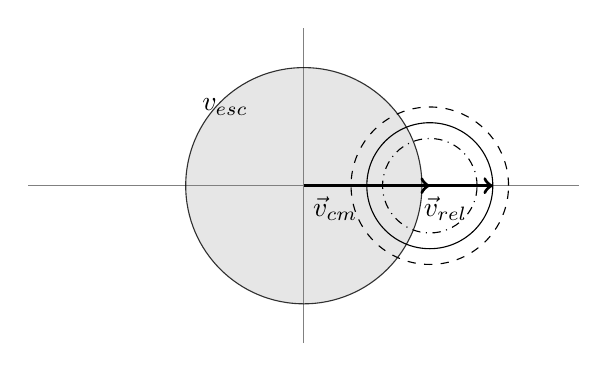
\begin{tikzpicture}
	
	\draw [gray] (-3.5,0) -- (3.5,0);
	\draw [gray] (0,-2) -- (0,2);
	
	\filldraw [ draw=black, fill=gray, draw opacity = 0.8,fill opacity=0.2] (0,0) circle (1.5);
	\node at (-1,1) {$v_{esc}$};
	
	%\filldraw[black] (1.2,0) circle (1.5pt) node [anchor = east]{$v_{cm}$};
	\draw[very thick,->] (0,0) -- (1.6,0) node [near start,below]{$\vec{v}_{cm}$};
	\draw[very thick,->] (0,0) -- (2.4,0) node [near end,below]{$\vec{v}_{rel}$};
	\draw[] (1.6,0) circle (0.8);
	\draw[dashed,draw=black] (1.6,0) circle (1.0);
	\draw[dashdotted,draw=black] (1.6,0) circle (0.6);
\end{tikzpicture}
\end{subfigure}
\begin{subfigure}[b!]{0.45\textwidth}
	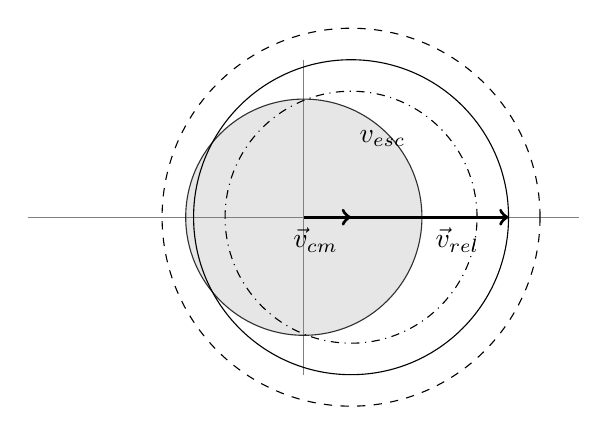
\begin{tikzpicture}
		
		\draw [gray] (-3.5,0) -- (3.5,0);
		\draw [gray] (0,-2) -- (0,2);
		
		\filldraw [ draw=black, fill=gray, draw opacity = 0.8,fill opacity=0.2] (0,0) circle (1.5);
		\node at (1,1) {$v_{esc}$};
		
		%\filldraw[black] (1.2,0) circle (1.5pt) node [anchor = east]{$v_{cm}$};
		\draw[very thick,->] (0,0) -- (0.6,0) node [near start,below]{$\vec{v}_{cm}$};
		\draw[very thick,->] (0,0) -- (2.6,0) node [near end,below]{$\vec{v}_{rel}$};
		\draw[] (0.6,0) circle (2);
		\draw[dashed,draw=black] (0.6,0) circle (2.4);
		\draw[dashdotted,draw=black] (0.6,0) circle (1.6);
	\end{tikzpicture}
\end{subfigure}
\caption {Кинематика соударения, слева $m_N < m_{\chi}$, справа $m_N > m_{\chi}$}
\label{pic:capture}
\end{figure}

Полная скорость захвата определяется суммой скоростей захвата для каждого элемента. Их концентрация определяется из соответствующей модели небесного тела. Для Солнца это AGSS09 \cite{Vinyoles_2017}, для Земли --- PREM \cite{DZIEWONSKI1981297}

%H	73.4
%He	25.0
%O	0.8
%C	0.20
%C	0.20
%N	0.09
%Si	0.09
%\iffalse
\begin{table}[h!]
	\centering
	\begin{tabular}{|c|c||c|c|}
		\hline
		\multicolumn{2}{|c||}{\text{Солнце}} & \multicolumn{2}{c|}{\text{Земля}}\\
		\hline
		Элемент & м.д. & Элемент & м.д.\\ 
		\hline
		H &	0.73 & Fe & 0.56\\ 
		\hline
		He & 0.25 & O & 0.15\\
		\hline
		O &	0.008 & Si & 0.13\\
		\hline
		C &	0.002 & Mg & 0.10\\
		\hline
		Fe & 0.0014 & S & 0.03\\
		\hline
	\end{tabular}
	\label{tab:mass_fractions}
	\caption{Массовые доли основных элементов на Солнце и Земле}
\end{table}
%\fi

После захвата темная материя термализуется и аннигилирует. Тогда полное число частиц удовлетворяет уравнению
\begin{equation}
	\label{eq:evolve_big}
	\tderiv{N} = C - A N^2
\end{equation}
где $C$ --- захват, $AN^2$ --- аннигиляция.

Решением этого уравнения является
\begin{equation}
	N = \sqrt{\cfrac{C}{A}}\tanh{\cfrac{t}{t_0}}
\end{equation}
где $t_{0} = (AC)^{-\frac{1}{2}}$.

Существует два предельных случая поведения этого уравнения: когда преобладает захват и $N = Ct$, либо когда система находится в равновесии и $N = \sqrt{\frac{C}{A}}$, тогда скорость аннигиляции равна скорости захвата.
Распределение по радиусу при этом считается термальным и имеет, согласно H-теореме Больцмана, следующий вид
\begin{equation}
	\label{eq:therm_dens}
	f(r) d^3\vec{r} = n_0\exp(-\frac{m\phi(r)}{2T_0})d^3\vec{r} \approx
	 n_1\exp(-\frac{r^2}{r_0^2})d^3\vec{r}
\end{equation}
(потенциал приближается квадратичной формой)



\section{Генерация потоков нейтрино}

Зная количество частиц внутри небесного тела и темп аннигиляции, определяется спектр нейтрино. При этом аннигиляция идет по каналу $f$ (это могут быть нейтрино $\nu\overline{\nu}$, кварки $b\overline{b}, t\overline{t}, \tau\overline{\tau}$ в случае s-канальной аннигиляции или бозоны $W^+W^-, ZZ$, $hh$ в случае t-канальной). Нейтрино образуется в результате распада этих промежуточных состояний \cite{CIRELLI2008338}
\begin{equation}
	\cfrac{d N_{\nu}}{d E_{\nu}} = \cfrac{\Gamma_{ann}}{4\pi L^2} \sum_f{p_f \cfrac{d N^f_{\nu}}{d E_{\nu}}}
\end{equation}
где $L$ --- расстояние до детектора, $p_f$ --- доля канала $f$ в аннигиляции.

\begin{figure}[!h]
	\centering
	\begin{subfigure}[b!]{0.3\textwidth}
		\begin{tikzpicture}
			
			\draw [] (-1,-1) -- (0,0) node [near start,above]{$\chi$};
			\draw [] (-1,1) -- (0,0) node [near start,above]{$\chi$};
			\draw [] (0,0) -- (2,0);
			
			\draw [] (3,-1) -- (2,0) node [near start,above]{$q$};
			\draw [] (3,1) -- (2,0) node [near start,above]{$\overline{q}$};

		\end{tikzpicture}
	\end{subfigure}
	\begin{subfigure}[b!]{0.2\textwidth}
		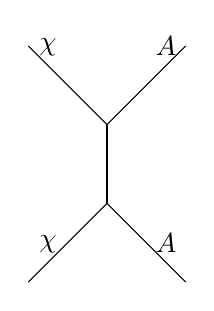
\begin{tikzpicture}
			
			\draw [] (-1,-1) -- (0,0) node [near start,above]{$\chi$};
			\draw [] (-1,2) -- (0,1) node [near start,above]{$\chi$};
			\draw [] (0,0) -- (0,1);
			
			\draw [] (1,-1) -- (0,0) node [near start,above]{$A$};
			\draw [] (1,2) -- (0,1) node [near start,above]{$A$};
		\end{tikzpicture}
	\end{subfigure}
	\caption {Аннигиляция в кварки и бозоны}
	\label{pic:ann_channels}
\end{figure}

Эти потоки нейтрино достигают детектора и дают события регистрации нейтрино. Вероятность зарегистрировать нейтрино пропорциональна числу актов аннигиляции $\Gamma_{ann}$, происходящих внутри небесного тела. Поэтому отутствие сигнала в конкретном детекторе приводит к ограничению темпа аннигиляции $\Gamma_{ann}$. 
Мы будем использовать ограничения из IceCube \cite{Aartsen_2017} на темп аннигиляции для ограничения сечения.


